\subsection{Modular protocol for 2PC (GMW protocol)}

Yao's protocol uses special encryption, and does not generalize to $n > 2$
parties. GMW (Goldreich, MIcali, Wigderson) uses only $\operatorname{XOR}$
operations, and is information-theoretically secure. Uses OT as a black box.

Idea:
\begin{itemize}
		\item Use $2-of-2$ secret sharing for each value on wire in $C$: $x
				\leftrightarrow (r, r \oplus x) = (s_A, S_B)$ where $r \rgets
				\{0, 1\}$, $s_A$ given to $A$, $s_B$ to $B$ are shares of $r$
		\item Use OT to evluate each gate in $C$
\end{itemize}

\subsubsection{Sharing inputs}

\begin{itemize}
		\item Parties $A(x)$, $B(y)$ with $x, y$ of length $l$
		\item Circuit $C$ of $f(x, y)$ consisting of NOT, XOR, AND gates
		\item A: Share inputs: $s^A_j \rgets \{0, 1\}, s^B_j \coloneqq x \oplus
				s^A_j$ for $j = 1 \ldots l$
		\item A: Send all of B's shares $s^B_i$ to $B$
		\item B: Share inputs: $s^A_{j+l} \rgets \{0, 1\}, s^B_{j+l} \coloneqq x \oplus
				s^A_{j+l}$ for $j = 1 \ldots l$
				\begin{itemize}
						\item Note how wire indices shifted, just so we don't
								have an index conflict of shares for inputs of
								$A$ and $B$. Alternative notation would
								introduce third index per share.
				\end{itemize}
		\item $A$ and $B$ now have one share each for all the inputs.
\end{itemize}

\subsubsection{Evaluating XOR gates}

For every gate in $C$ in some topological order, evaluate as follows:

\paragraph{XOR gates}

$w_t = w_i \oplus w_j$, where:
\begin{itemize}
		\item $A$ holds $s^A_i, s^A_j$, $B$ holds $s^B_i, s^B_j$
		\item Such that $s^A_i \oplus s^B_i = w_j$, $s^A_j \oplus s^B_j = w_j$
\end{itemize}

Now:
\begin{align*}
		w_t & = w_i \oplus w_j \\
			& = (s^A_i \oplus s^B_i) \oplus (s^A_j \oplus s^B_j) \\
			& = (s^A_i \oplus s^A_j) \oplus (s^B_i \oplus s^B_j) \\
			& = s^A_t \oplus s^B_t
\end{align*}

So $A$ can compute $s^A_t$, $B$ can compute $s^B_t$ locally, and each now have
a share of the output wire $w_t$.

\paragraph{NOT gates}

$w_t = \neg w_i$, where:
\begin{itemize}
		\item $A$ has $s^A_i$, $B$ has $s^B_i$
		\item Such that $w_i = s^A_i \oplus s^B_i$
\end{itemize}

Now:
\begin{itemize}
		\item $A$ sets $w^A_t \coloneqq s^A_i \oplus 1$
		\item $B$ sets $w^B_t \coloneqq s^B_i$
\end{itemize}

Then $w_t = w^A_t \oplus w^B_t$, so both have a valid share again using only
local operations.

\paragraph{AND gates}

$w_t = w_i \land w_j$, where:
\begin{itemize}
		\item $A$ holds $s^A_i, s^A_j$, $B$ holds $s^B_i, s^B_j$
		\item Such that $s^A_i \oplus s^B_i = w_j$, $s^A_j \oplus s^B_j = w_j$
\end{itemize}

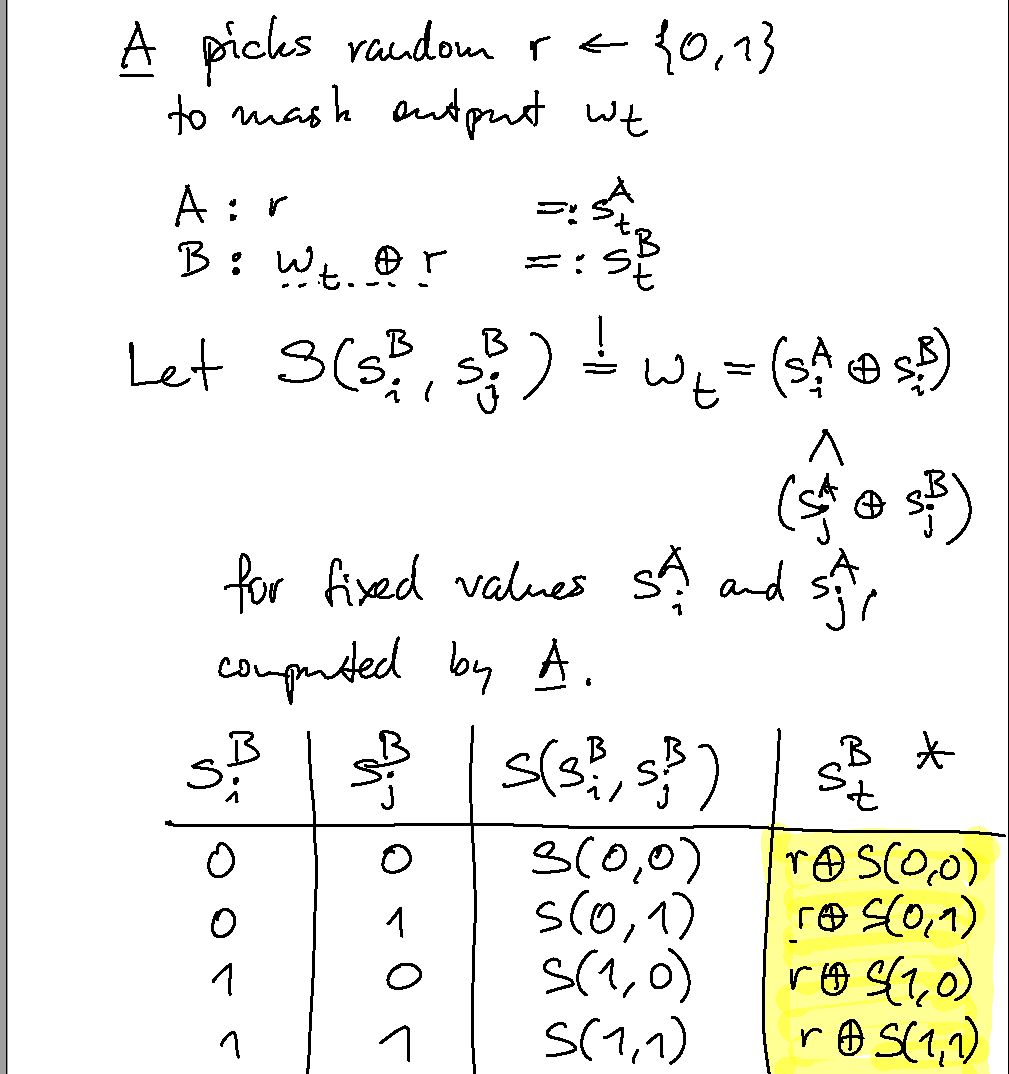
\includegraphics[width=0.7\textwidth]{9_and_1}

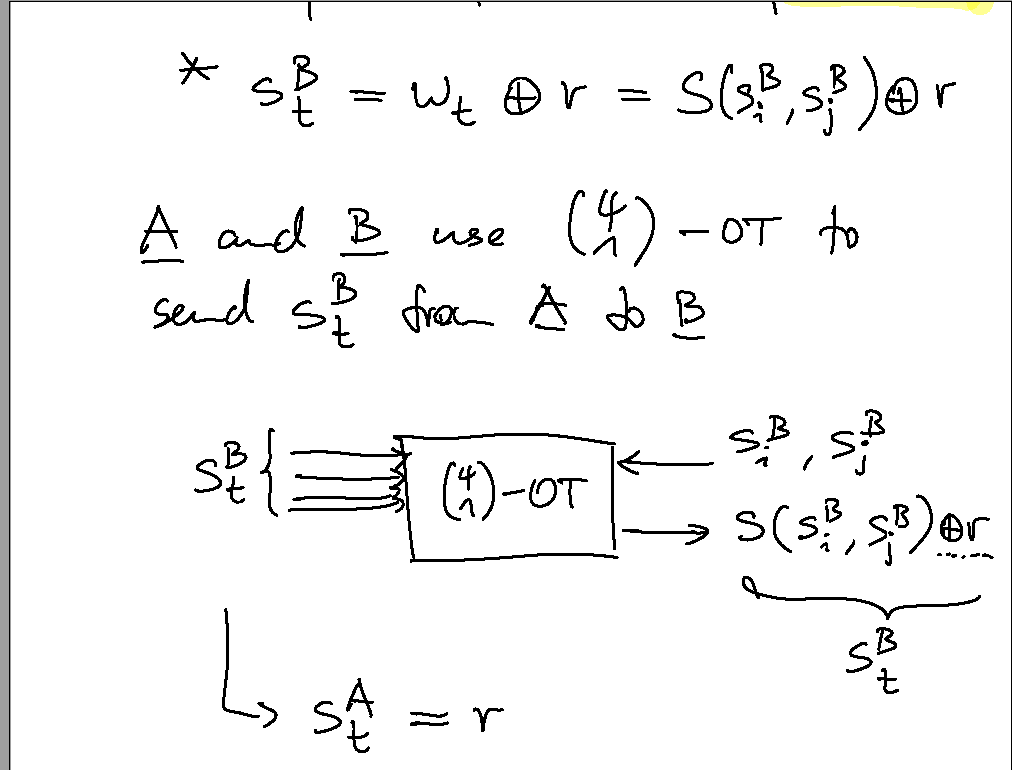
\includegraphics[width=0.7\textwidth]{9_and_2}

\paragraph{Output wires}

\begin{itemize}
		\item A: send ${s^A_o}$ for every output wire $o$ to $B$.
		\item B: $w_o \coloneqq s^A_o \oplus s^B_o$
		\item B: send ${s^B_o}$ for every output wire $o$ to $B$.
		\item A: $w_o \coloneqq s^A_o \oplus s^B_o$
\end{itemize}

Now $A$, $B$ have both reconstructed the values of the output wires.

\paragraph{Cost}

\begin{description}
		\item[Pk-Operations] $O(|C|)$
		\item[Communication bits] $O(|C|)$
		\item[Latency] $O(depth(C))$, higher than Yao's.
\end{description}

Depth is longest path from any input to an output, counting AND gates.

\subsection{Generalisation to $n$ parties $P_1, \ldots P_n$}

Idea: Use additive sharing of secret in $n-out-of-n$ model, $x \leftrightarrow
(x_1, \ldots x_n)$, with $x_i$ given to $P_i$.

Then $w_i$ on wire $i$ is represented by shares $s_1, \ldots, s_n$: $w_i
\leftrightarrow (s^1_i, \ldots, s^n_i)$

Protocol as before, except for AND gates. There:
\begin{align*}
		w_t & = w_i \land w_j \\
			& = (\oplus_{k=1}^n s^k_i) \land (\oplus_{k=1}^n s^k_j) \\
			& = (\oplus_{k=1}^n s^k_i \land s^k_j) \oplus (\oplus_{k, l = 1, k \neq l}^n s^k_i \land s^l_j) \\
\end{align*}

Note how first $\oplus$ operation is those with same lower index, second one
all those with differing ones.

\begin{itemize}
		\item $P_k$ can compute $s^k_i \land s^k_j$ locally
		\item $P_k, P_l$ can compute a 2-of-2-sharing of $s^k_i \land s^l_j$
				using 2-party protocol step with a $4-1 OT$ as before
		\item In the end, $P_1, \ldots, P_n$ again have additive shares of $w_t \leftrightarrow (s^1_t, \ldots s^n_t)$
		\item Using $n \cdot (n - 1)$ OT protocols
\end{itemize}

\section{Distributed cryptography}

Idea: Cryptography with e.g $n = 9$, $t = 4$, secure as long as no more than
$t$ of the parties are corrupted.

\subsection{Secret sharing}

Share secret $s$ among parties $P_1, \ldots, \P_n$ such that any $t+1$ parties
can recover it, and no $t$ (or fewer) parties have any information on $s$.

\begin{itemize}
		\item Dealer picks random polynomial $f(x)$ over $GF(q)$ of degree $t$,
				such that $f(0) = s$: $f(x) = \sum_{i=1}^t f_i \cdot x^i + s$
		\item D gives $s_i = f(i)$ to $P_i$
		\item From any $t+1$ points, the polynomial, and therefore $s = f(0)$, can be recovered
\end{itemize}

Note:
\begin{align*}
		s & = f(0) \\
		  & = \sum_{i \in S} \lambda^S_{0, i} \cdot s_i
\end{align*}

Where:
\begin{align*}
		\lambda^S_{0, i} & = \prod_{j \in S, j \neq i} \frac{j}{j-i}
\end{align*}

Is the simplified (for $x = 0$) lagrange base polynomial.
